\newcommand{\xbold}{{\bf x}}
\newcommand{\ibold}{{\bf i}}
\newcommand{\jbold}{{\bf j}}
\newcommand{\kbold}{{\bf k}}
\newcommand{\nbold}{{\bf k}}
\newcommand{\cbold}{{\bf k}}
\newcommand{\ebis}{{\tt EBIndexSpace}}
\newcommand{\baseif}{{\tt BaseIF}}
\newcommand{\sphereif}{{\tt SphereIF}}
\newcommand{\transformif}{{\tt TransformIF}}
\newcommand{\latheif}{{\tt LatheIF}}
\newcommand{\unionif}{{\tt UnionIF}}
\newcommand{\intersectionif}{{\tt IntersectionIF}}
\newcommand{\geom}{{\tt GeometryShop}}
\newcommand{\parm}{{\tt ParmParse}}

\section{Overview of Embedded Boundary Description}
\label{sec:EB:EBOverview}

For computations with complex geometries, $\tt{AMReX}$ provides data
structures and algorithms to employ an embedded boundary (EB) approach to
PDE discretizations.    In this approach, the underlying computational
mesh is uniform and block-structured, but the boundary of the irregular-shaped
computational domain conceptually cuts through this mesh.  Each cell in the mesh
becomes labeled as regular, cut or covered, and the finite-volume based
discretization methods traditionally used in AMReX applications can be
modified to incorporate these cell shapes.  See Figure~\ref{fig::ebexample}
for an illustration.
\begin{figure}[h]
  \centering
  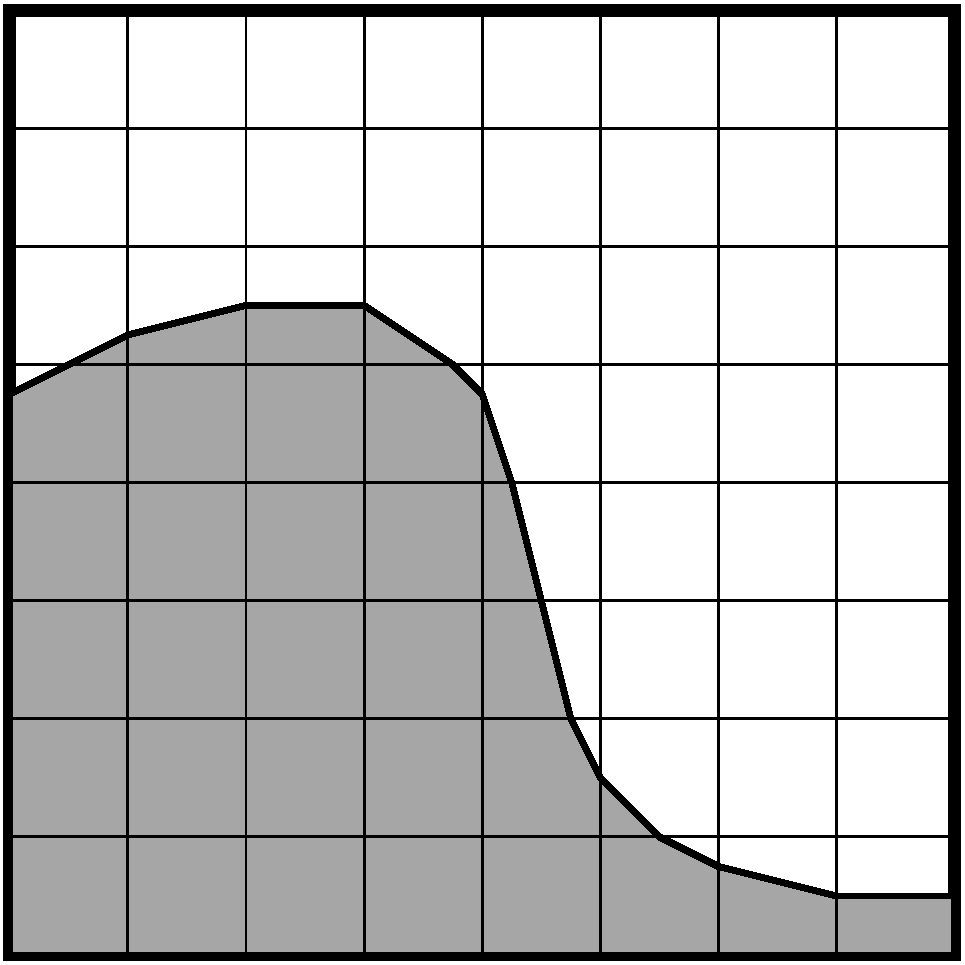
\includegraphics[width=0.25\textwidth]{./EB/EB_example.pdf}
  \caption{\label{fig::ebexample}In the embedded boundary approach to
    discretizing PDEs, the (uniform) rectangular mesh is cut by the
    irregular shape of the computational domain.  The cells in the
    mesh are label as regular, cut or covered.}
\end{figure}
Because this is a relatively simple grid
generation technique, computational meshes for rather complex geometries
can be generated quickly and robustly.  However, the technique 
can produce arbitrarily small cut cells in the domain.  In practice such small
cells can have significant impact on the robustness and stability of
traditional finite volume methods.  In this chapter we overview
a class of approaches to deal with this ``small cell'' problem in a
robust and efficient way, and discuss the tools and data that $\tt{AMReX}$
provides in order to implement them.  

Note that in a completely general implementation of the EB approach, 
there would be no restrictions on the shape or complexity of the EB surface.  
With this generality comes the possibility that the process of "cutting" the cells
results in a single $(i,j,k$) cell being broken into multiple cell fragments.
%In the block-structured context of $\tt{AMReX}$, this would trigger a significant complication
%because the state data (as well as the geometrical and cell
%connectivity information) can no longer be managed using the logically rectangular
%data structures with implied connectivity graphs that are native to the framework.  Because of this,
The current release of $\tt{AMReX}$ does not support multi-valued cells, thus there is a
practical restriction on the complexity of domains (and numerical algorithms) supported.  
AMReX support for EB with AMR will be available by early 2018;
EB support for multi-valued cells will follow.
%as it leads to complexities in data communication patterns
%and inter-level data transfer operations.  
%In both cases however, extended support is
%planned for future releases of the library, and the software infrastructure
%underlying the implementation described in this document have been designed with these
%extensions in mind.

This chapter discusses the EB tools, data structures and algorithms currently supported by
$\tt{AMReX}$ to enable the construction of discretizations of conservation law systems.
The discussion will focus on general requirements associated with building fluxes and
taking divergences of them to advance such systems.  We also give examples of how to
initialize the geometry data structures and access them to build the numerical difference
operators.

\subsection{Finite Volume Discretizations}
Consider a system of PDEs to advance a conserved quantity $U$
with fluxes $F$:
\begin{equation}
\frac{\partial U}{\partial t} + \nabla \cdot F = 0.
\label{eqn::hypsys}
\end{equation}
A conservative, finite volume discretization starts with
the divergence theorm
$$
\int_V \nabla \cdot F dV = \int_{\partial V} F \cdot n dA.
$$
In an embedded boundary cell, the ``conservative divergence'' is discretized  (as
$D^c(F)$) as follows
\begin{equation}
D^c(F) = \frac{1}{\kappa h} \left( \sum^D_{d = 1}
  (F_{d, hi}A_{d,hi} - F_{d, lo}A_{d,lo})  + F^{EB} A^{EB} \right).
\label{eqn::ebdiv}
\end{equation}

Geometry is discretely represented by volumes ($V = \kappa h^d$) and apertures 
($A= \alpha h^{d-1}$), where $h$ is the (uniform) mesh spacing at that AMR level,
$\kappa$ is the volume fraction and $\alpha$ are the area fractions.
Without multivalued cells the volume fractions, area fractions and cell and face centroids 
(see Figure~\ref{fig::volume}) are the only geometric information needed to 
compute second-order fluxes centered at the face centroids,  
and to infer the connectivity of the cells.  
Cells are connected if adjacent on the Cartesian mesh, and only via
coordinate-aligned faces on the mesh.  If an aperture, $\alpha = 0$, between two
cells, they are not directly connected to each other.

\begin{figure}[h]
  \centering
  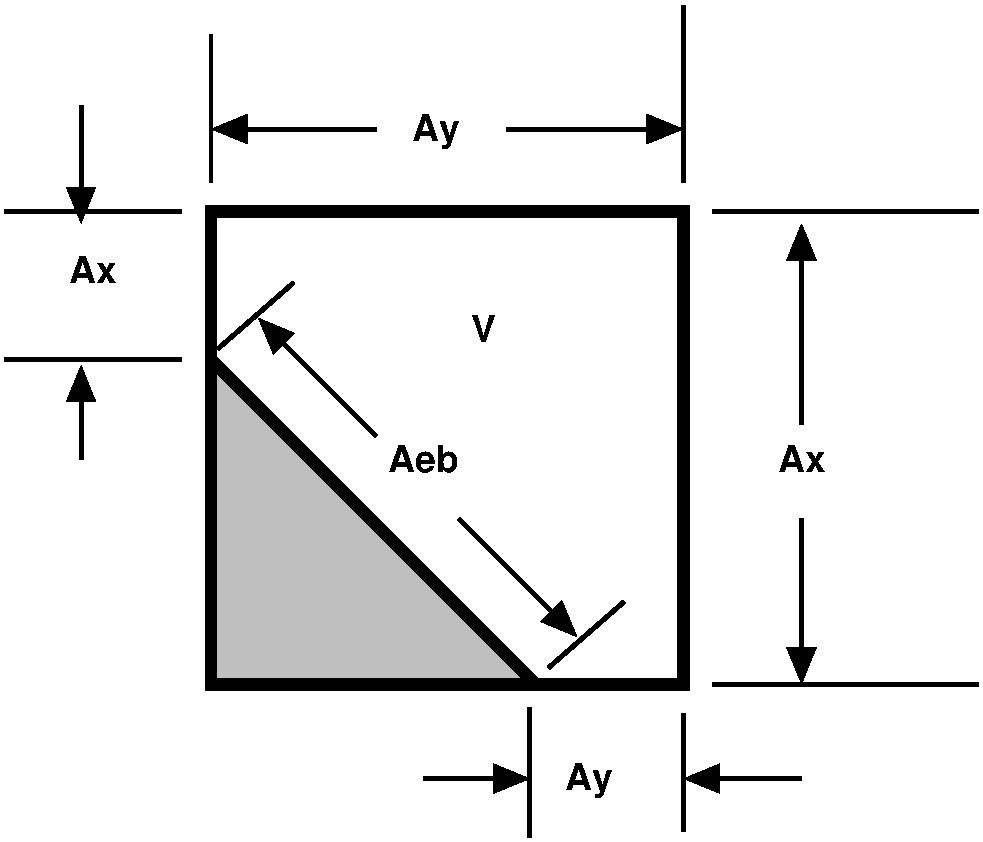
\includegraphics[width=0.25\textwidth]{./EB/areas_and_volumes.pdf}
  \hspace{1in} 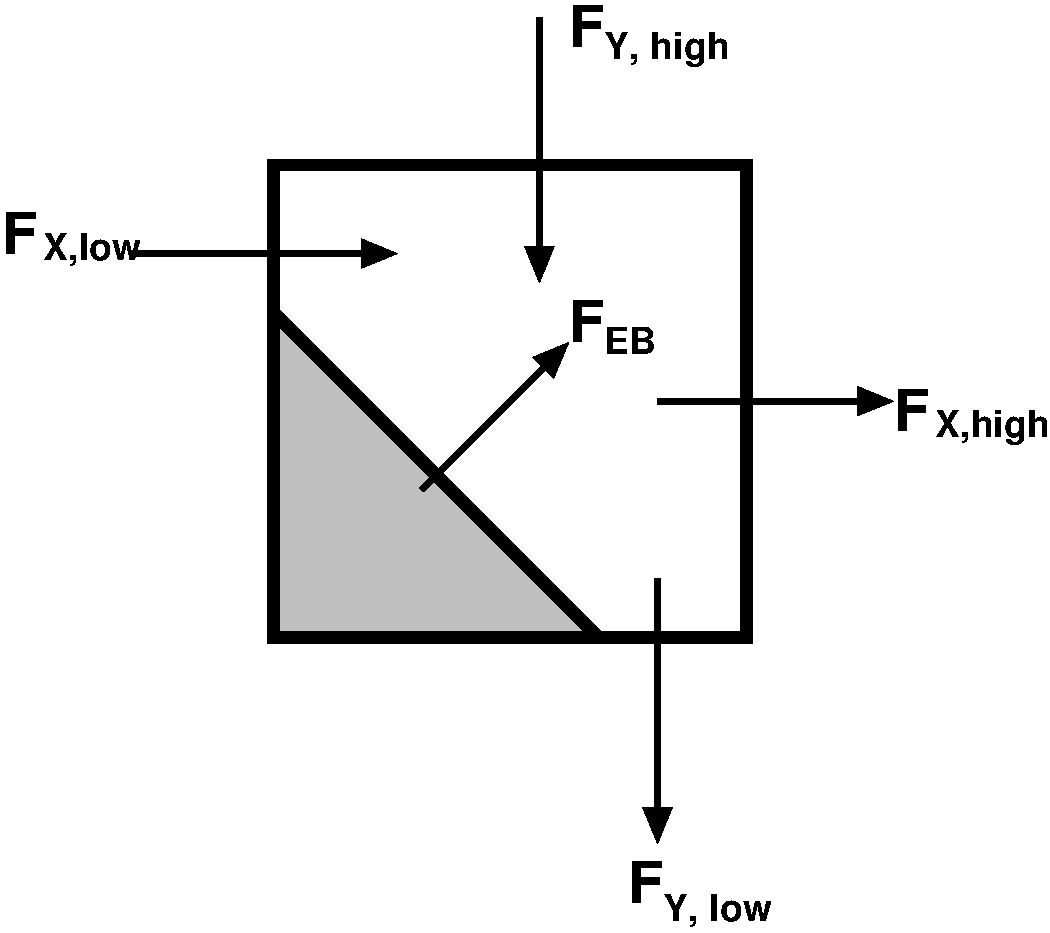
\includegraphics[width=0.25\textwidth]{./EB/eb_fluxes.pdf}
  \caption{\label{fig::volume} (a) A typical two-dimensional uniform cell that is cut by the embedded
    boundary. The grey area represents the region excluded from the calculation.   The
    portion of the cell faces (labelled with A) through which fluxes flow are the ``uncovered''
    regions of the full cell faces.  The volume (labelled V) is the uncovered
    region of the interior. (b) Fluxes in a cut cell.}
\end{figure}
%\begin{figure}[h]
%  \centering
%  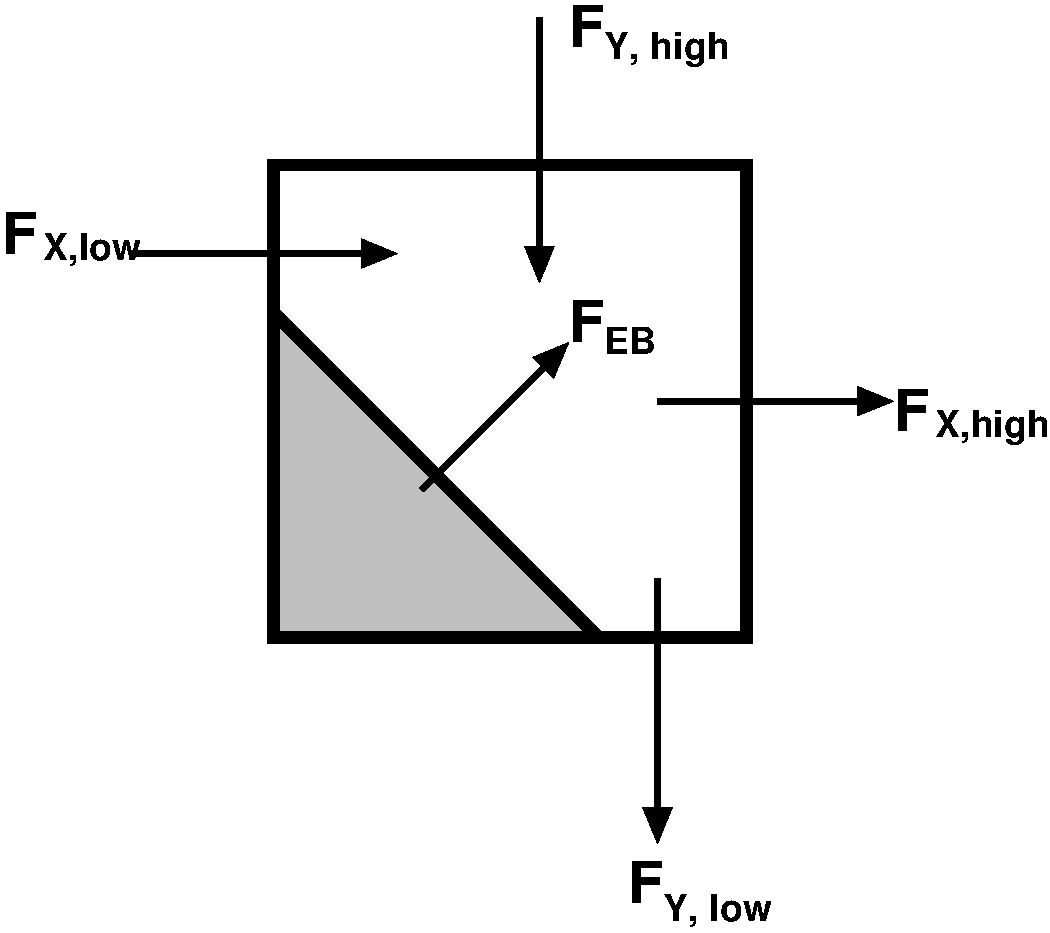
\includegraphics[width=0.25\textwidth]{./EB/eb_fluxes.pdf}
%  \caption{\label{fig::eb_fluxes}The divergence of fluxes in a cut cell.}
%\end{figure}
%\begin{itemize}
%\item
%Volume fractions,
%\item
%Area fractions,
%\item 
%Cell and face centroids
%\end{itemize}

\subsection{Small Cells And Stability}

In the context of time-explicit advance methods for, say hyperbolic conservation laws, 
a naive discretization in time of \ref{eqn::hypsys} using \ref{eqn::ebdiv},
$$
U^{n+1} = U^{n} - \delta t D^c(F)
$$
would have a time step constraint $\dt \sim h \kappa^{1/D}/V_m$,  which
goes to zero as the size of the 
smallest volume fraction $\kappa$ in the calculation.  Since EB volume fractions can
be arbitrarily small, this is an unacceptable constraint.  One way to remedy
this is to create ``non-conservative'' approximation to the divergence
$D^{nc}$, which at a cell $\ibold$, can be formed as an average of the conservative
divergences in the neighborhodd, $N_\ibold$, of $\ibold$.
$$
D^{nc}(F)_\ibold = \frac{\sum_{\jbold \in N_\ibold}\kappa_\jbold D(F)_\jbold}{\sum_{\jbold \in N_\ibold}\kappa_\jbold}
$$
Incorporating this form, the solution can be updated using a {\it hybrid divergence},
$D^H(F) = \kappa D^c(F) + (1-\kappa)D^{nc}$:
$$
U^{n+1,*} = U^n - \delta t D^H(F)
$$
However, we would like our finite-volume scheme to strictly conserve the field quantities
over the domain.  To enforce this, we calculate $\delta M$, the mass gained or
lost by not using $D^c$ directly,
$$
\delta M_\ibold = \kappa (1-\kappa)(D^c(F)_\ibold - D^{nc}(F)_\ibold)
$$
This ``excess material'' (mass, if $U=\rho$) can be {\em redistributed}\ in a time-explicit fashion
to neighboring cells, $\jbold \in N_\ibold$:
$$
\delta M_\ibold = \sum_{\jbold \in N_\ibold} \delta M_{\jbold, \ibold}.
$$
in order to preserve strict conservation over $N_\ibold$.

Note that the physics at hand may impact the optimal choice of precisely how the excess mass is distributed
in this fashion.  We introduce a weighting for redistribution, $W$,
\begin{equation}
\delta M_{\jbold, \ibold} =  \frac{\delta M_\ibold \kappa_\jbold
  W_\jbold}{\sum_{\kbold \in N_\ibold} \kappa_\kbold W_\kbold}
\label{eqn::massweight}
\end{equation}
For all $\jbold \in N_\ibold$,
$$
U^{n+1}_\jbold = U^{n+1,*}_\jbold + 
 \frac{\delta M_\ibold
  W_\jbold}{\sum_{\kbold \in N_\ibold} \kappa_\kbold W_\kbold}.
$$
 Typically, the redistribution neighborhood for each cell is one that can be reached via a monotonic
 path in each coordinate direction of unit length
(see, e.g., Figure~\ref{fig::redistribution})
\begin{figure}[h]
  \centering
  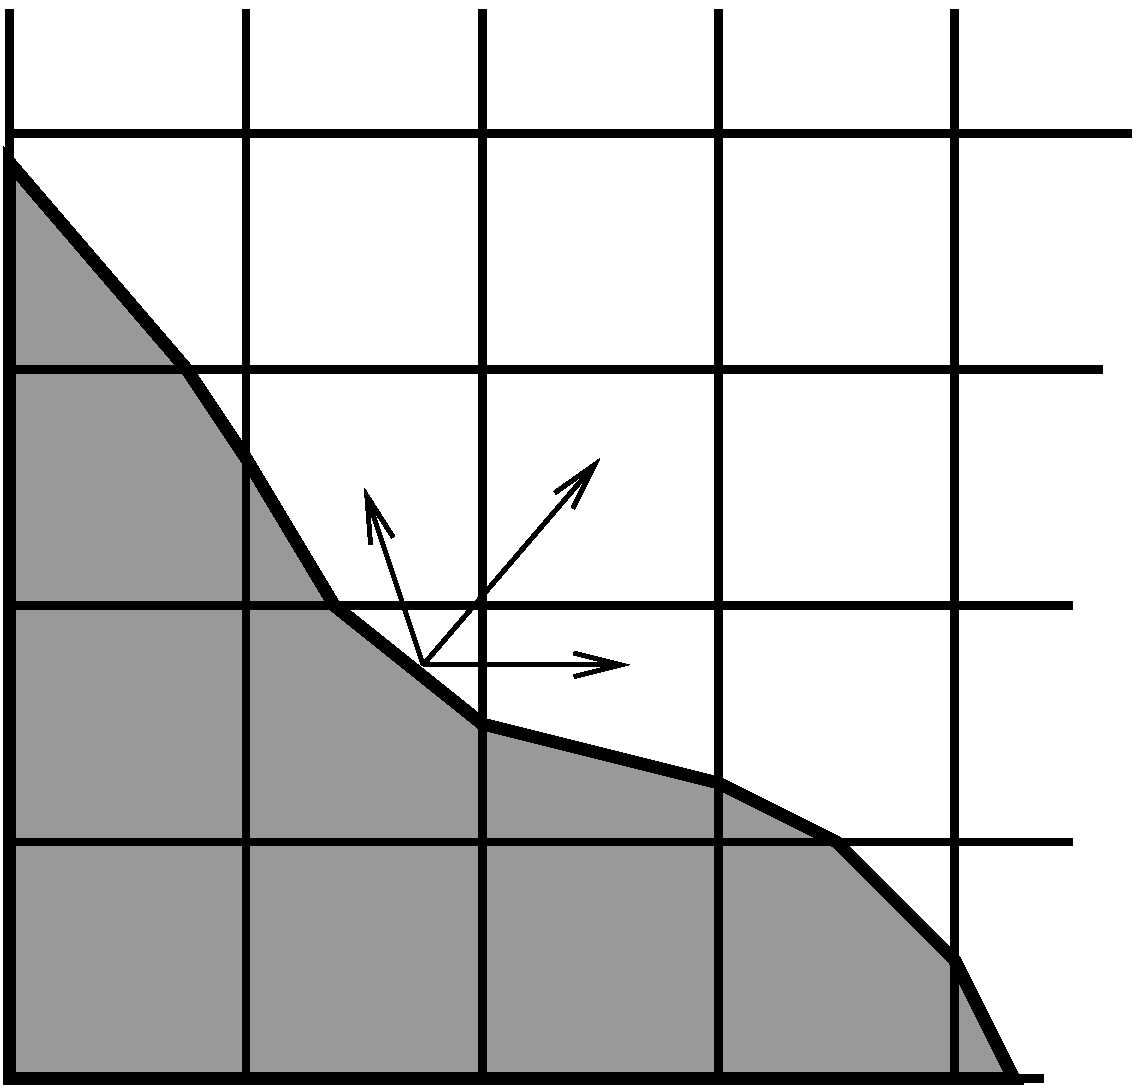
\includegraphics[width=0.25\textwidth]{./EB/redist.pdf}
\caption{\label{fig::redistribution}
Redistribution illustration.  Excess mass due to using a hybrid
divergence $D^H$ instead of the conservative divergence $D^C$ is
distributed to neighbor cells.}
\end{figure}

\section{Initializing \ebis, the Geometric Database}
\label{sec:EB:ebinit}

In $\tt{AMReX}$ the geometric information is stored in a distributed database class, \ebis, which must be
initialized at the start of the calculation.  The procedure for this
goes as follows:
\begin{itemize}
\item Define function of position which describes the surface 
      and use it define a \geom\ object (see \S
      \ref{sec:EB:geometryshop}) -- specifically, the scalar value returned by this function takes on a
      negative value inside the fluid, a positive value in the body, and identically zero at the EB.
\item Construct an \ebis\ with the \geom\ object.   This
  will fill the underlying database of geometric information, specifically tailored to the
  actual meshes that will be used.  Thus, the construction requires one to specify
  the actual mesh resolution that will be used in a calculation.
\end{itemize}

To facilitate the first step, $\tt{AMReX}$ defines a virtual class, an ``implicit function'', \baseif, which encapsulates this functionality.
An instance of a \baseif\ object is required for the construction of a \geom\ object.
\begin{lstlisting}[language=cpp]
    GeometryShop(const BaseIF& a_localGeom)
\end{lstlisting}
Although the user is free to define their own instance of this class, $\tt{AMReX}$ provides a number of preconfigured useful ones.  This
are listed in the next section.

\subsection{Example: Spherical EB}
The spherical implicit function, \sphereif, derives from \baseif, and defines the function
$$
S(\xbold) = x^2 + y^2 + z^2 - R^2,
$$
In this case, the solution domain is defined as the interior of a sphere of radius $R$.
If the sign of $S$ is reversed, the solution domain is the exterior of the sphere.
The following example illustrates how to use the \sphereif\ class to define a \geom\ object:

\begin{lstlisting}[language=cpp]

  int nx = 1024;
  Box domain(IntVect::Zero, (nx-1)*IntVect::Unit);
  Real dx = 1.0/nx;
  Real radius = 0.1;
  Real center = 0.5*RealVect::Unit;
  bool insideRegular = false;
  //this is the implicit function
  SphereIF sphere(radius, center, insideRegular);

  //this is worker object that creates geometric information given an IF
  GeometryShop workshop(sideImpMultisphere)

  //this is the global, distributed database being initialized
  EBIndexSpace*  ebis = AMReX_EBIS::instance()
  ebis->define(domain, RealVect::Zero, dx, workshop);

\end{lstlisting}

In this case, we construct an $r=0.1$ sphere, centered within a unit cube.  The mesh resolution is $1024^3$.
The \geom\ object based on this sphere is then used to construct the \ebis, as shown.

\subsubsection{Other basic shapes:}

\begin{itemize}

\item Planes are made using the class $\tt{PlaneIF}$ which given a normal
$\nbold$  and a center $\cbold$ gives the implicit function 
$$
I(\xbold) = \sum_{1<=d<=D} n_d (x_d - c_d).
$$

\begin{lstlisting}[language=cpp]
RealVect normal; 
RealVect center;
...fill in values for n and c...

PlaneIF plane(normal,point, true);
GeometryShop workshop(plane)

EBIndexSpace*  ebis = AMReX_EBIS::instance()
ebis->define(domain, RealVect::Zero, dx, workshop);

\end{lstlisting}

\item Polynomials of any form can be made using the class
  $\tt{PolynomialIF}$.  Here is an example that makes a parabola of
  the form $I(\xbold) = x - y^2 - z^2$. 
\begin{lstlisting}[language=cpp]

Vector<PolyTerm> poly;
PolyTerm mono;
Real coef;
IntVect powers;
Real amplitude = 1;
// y^2 term
coef = amplitude;
powers = IntVect::Zero;
powers[1] = 2;

mono.coef   = coef;
mono.powers = powers;
poly.push_back(mono);

// z^2 term
coef = amplitude;
            RealVect translation;
      
            for(int idir = 0; idir < SpaceDim; idir++)
            {
              int finesize = finest_domain.size()[idir];
              translation[idir] = 0.5*finesize*fine_dx;
            }
            translation[0] = 0;

            TransformIF implicit(mirror);
            implicit.translate(translation);
            impfunc.reset(implicit.newImplicitFunction());

powers = IntVect::Zero;
powers[2] = 2;
mono.coef   = coef;
mono.powers = powers;
poly.push_back(mono);

// x term
coef = -1.0;
powers = IntVect::Zero;
powers[0] = 1;
mono.coef   = coef;
mono.powers = powers;

poly.push_back(mono);

PolynomialIF mirror(poly,false);
GeometryShop workshop(mirror)
EBIndexSpace*  ebis = AMReX_EBIS::instance()
ebis->define(domain, RealVect::Zero, dx, workshop);
\end{lstlisting}

\end{itemize}
\subsection{Implicit Function Transformation Tools}

More complex domains can be constructed by composing these fundamental shapes.
$\tt{AMReX}$ contains the following classes to compose implicit functions:
\begin{itemize}
\item $\tt{TransformIF}$    allows for translations and rotations of an implicit function.
\item $\tt{UnionIF}$        produces the union of two implicit functions.  
\item $\tt{IntersectionIF}$ produces the intersection of two implicit functions.
\item $\tt{LatheIF}$        creates a 3D implicit function as the surface of
  revolution of a 2D implicit function.
\end{itemize}

\subsection{Multi-sphere example}
The following example creates a geometry using multiple spheres:

\begin{lstlisting}[language=cpp]

vector<Real>     radius(numSpheres);
vector<RealVect> center(numSpheres);
...
//create an implicit function for each sphere
vector<BaseIF*>  spheres(numSpheres);

for(int isphere = 0; isphere < numSpheres; isphere++)
{
  // Create sphere at each origin and translate
  SphereIF sphereAtZero(radius[isphere], RealVect::Zero, false);
  TransformIF* movedSphere = new TransformIF(sphereAtZero);
  movedSphere->translate(center[isphere]);
  spheres[isphere] = static_cast<BaseIF*>(movedSphere);
}
// Create implicit function as intersection of spheres
IntersectionIF impMultisphere(spheres);

// Fluid will in the complement space outside the sphere
ComplementIF sideImpMultisphere(impMultisphere, false);

// Construct the geometryshop
GeometryShop workshop(sideImpMultisphere)
\end{lstlisting}

\subsection{Geometric example 2 -- Surface of revolution}

Here is an example that creates a geometric construction using a
surface of revolution of a set of polygons.   This particular example
only makes sense in three dimensions.   With the right polygons, it
creates the surface shown in \ref{fig::revolution}.

\begin{lstlisting}[language=cpp]

/// define EBIndexSpace from the surface of revolution of a set of polygons
void
defineGeometry(const Real& fine_dx, const  Box& finest_domain, int max_grid_size)
{
  amrex::Print() << "creating geometry from polygon surfaces of revolution" << endl;

  // These  the polygons that get built around the z axis
  Vector<Vector<RealVect> > polygons;
  //....fill the polygons any way you like//

  // Make the Array of (convex) polygons (Arrays of points) into a union
  // of convex polygons, each made from the intersection of a set of half
  // planes/spaces - all represented by implicit functions.

  // A list of all the polygons as implicit functions
  Vector<BaseIF*> polytopes;
  polytopes.resize(0);
  int numPolys = polygons.size();
  // Process each polygon
  for (int p = 0; p < numPolys; p++)
  {
    // All the half planes/spaces used to make a polygon
    Vector<BaseIF*> planes;
    planes.resize(0);

    // Get the current polygon (as a Array of points)
    const Vector<RealVect>& polygon = polygons[p];

    // Get the number of points in the polygon
    int numPts = polygon.size();

    // Process each pair of points
    for (int n = 0; n < numPts; n++)
    {
      // The normal and point is space used to specify each half plane/space
      RealVect normal(RealVect::Zero);
      RealVect point;

      // Set the normal remembering that the last point connects to the first
      // point.
      normal[0] = -(polygon[(n+1) % numPts][1] - polygon[n][1]);
      normal[1] =  (polygon[(n+1) % numPts][0] - polygon[n][0]);

      point = polygon[n];

      // Generate the appropriate half plane/space (as an implicit function)
      PlaneIF* plane;
      plane = new PlaneIF(normal,point,true);

      // Save the result
      planes.push_back(plane);
    }

    // Intersect all the half planes/spaces to create an implicit function
    // that represents the polygon
    IntersectionIF* polygonIF = new IntersectionIF(planes);

    polytopes.push_back(polygonIF);
  }

  //this makes the cross section the union of all the polgons (around
  //z-axis, recall)
  UnionIF crossSection(polytopes);
            
  // In 3D rotate about the z-axis 
  LatheIF lathe(crossSection, false);

  //we are starting around the z axis so we need to translate
  //over to the center of the x-y plane
            
  RealVect translation;
  for(int idir = 0; idir < SpaceDim; idir++)
  {
    translation[idir] = 0.5*finest_domain.size()[idir]*fine_dx;
  }
  translation[2] = 0;
  TransformIF implicit(lathe);
  implicit.translate(translation);

  //create a workshop from translated surface of revolution
  GeometryShop gshop(implicit, false);
  //define th geometric database
  AMReX_EBIS::instance()->define(finest_domain, RealVect::Zero,
                                 fine_dx, gshop, max_grid_size);
}

\end{lstlisting}

\begin{figure}[h]
  \centering
  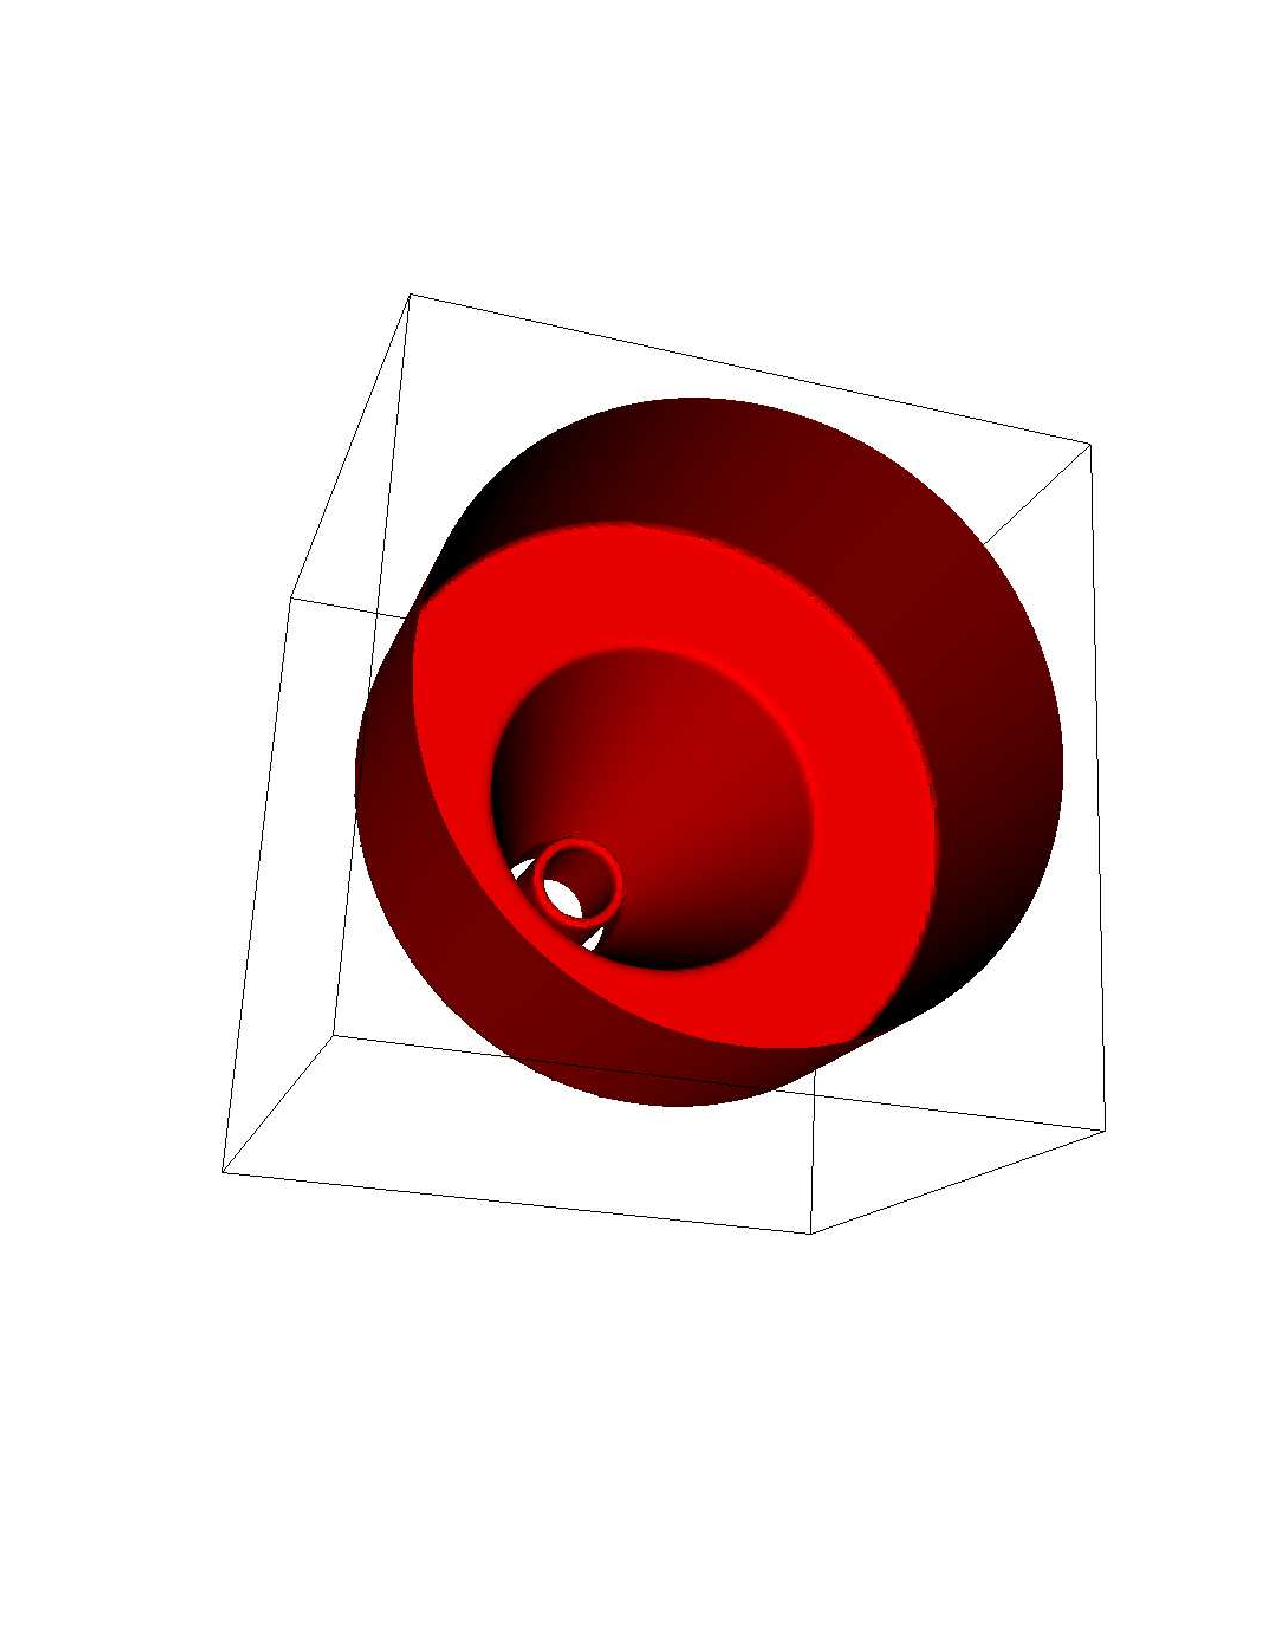
\includegraphics[width=0.375\textwidth]{./EB/revolution.pdf}
  \caption{\label{fig::revolution} Zero surface of an implicit
    function made using a surface of revolution.}
\end{figure}
\subsection{Geometric example 3 -- A Sphere Inside a Parabola}

Here is an example that creates a geometry of a sphere contained
within a parabola. This code
creates the surface shown in \ref{fig::parabolasphere}.

\begin{lstlisting}[language=cpp]
Vector<PolyTerm> poly;

PolyTerm mono;
Real coef;
IntVect powers;
Real amplitude = 1;

// y^2 term
coef = amplitude;
powers = IntVect::Zero;
powers[1] = 2;

mono.coef   = coef;
mono.powers = powers;

poly.push_back(mono);

// z^2 term
coef = amplitude;
powers = IntVect::Zero;
powers[2] = 2;
mono.coef   = coef;
mono.powers = powers;
poly.push_back(mono);

// x term
coef = -1.0;
powers = IntVect::Zero;
powers[0] = 1;
mono.coef   = coef;
mono.powers = powers;

poly.push_back(mono);

PolynomialIF mirror(poly,false);
RealVect translation;

for(int idir = 0; idir < SpaceDim; idir++)
{
  int finesize = finest_domain.size()[idir];
  translation[idir] = 0.5*finesize*fine_dx;
}
RealVect center = translation;
translation[0] = 0;

TransformIF transform(mirror);
transform.translate(translation);

Real radius = 0.2*center[0];
SphereIF sphere(radius, center, true);
Vector<BaseIF*> funcs(2);
funcs[0] = &transform;
funcs[1] = &sphere;
UnionIF implicit(funcs);
impfunc.reset(implicit.newImplicitFunction());
GeometryShop gshop(impfunc, false);
//define th geometric database
AMReX_EBIS::instance()->define(finest_domain, RealVect::Zero,
                                 fine_dx, gshop, max_grid_size);
\end{lstlisting}

\begin{figure}[h]
  \centering
  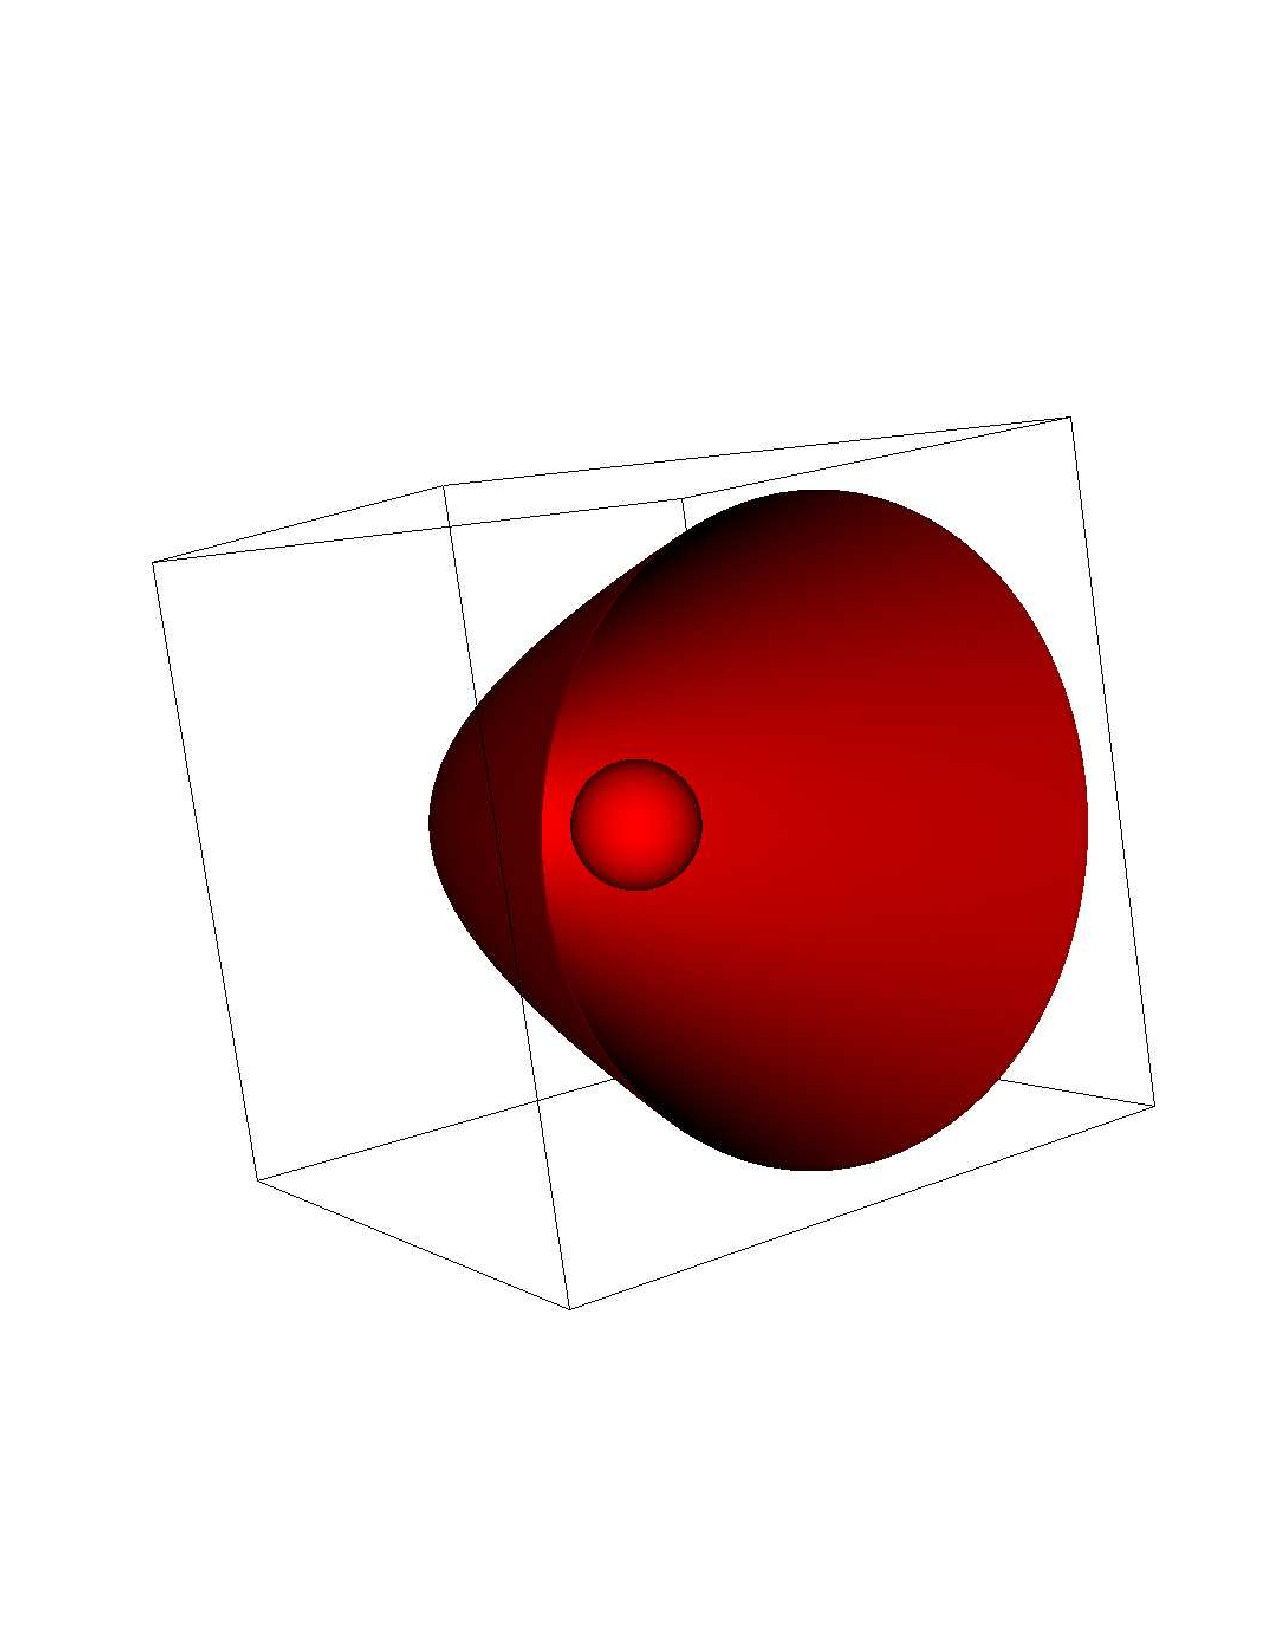
\includegraphics[width=0.375\textwidth]{./EB/parabsphere.pdf}
  \caption{\label{fig::parabolasphere} Zero surface of an implicit
    function made the above code.}
\end{figure}

\section{$\tt{EBFarrayBox}$}

The fundamental data structure for embedded boundary calculations is 
$\tt{EBFArrayBox}$. $\tt{EBFArrayBox}$ is an a $\tt{FArrayBox}$ with two extra
data members.
\begin{itemize}
\item $\tt{EBFArrayBox::getEBISBox}$ returns an $\tt{EBISBox}$, a data
  structure that contains the geometric information of an \ebis\ but
  restricted to a given box.
\item $\tt{EBFArrayBox::getEBCellFlagFab}$  is a
  $\tt{BaseFab<EBCellFlag>}$, where $\tt{EBCellFlag}$ is a class which
  is a class with tools that compactly specifies local cell connectivities
  on a box.
\end{itemize}
If one compiles with $\tt{AMREX\_USE\_EB = TRUE}$, the state data managed by
the ${\tt Amr}$ class is automatically of type $\tt{EBFArrayBox}$ (typically the data
is exposed explicitly as a $\tt{MultiFab}$, but the additional functionality
may be accessed through a C++ type cast. The
$\tt{EBCellFlagFab}$ can be used down in $\tt{Fortran}$, e.g., to choose
locally whether EB-specific operations and data are required for constructing
discretizations.  In the next section, we show examples of this workflow.

\subsection{$\tt{EBFarrayBox}$ Usage Example}
In order to make these EB concepts more concrete, we discuss here sample code
that appears in the $\tt{AMReX}$ tutorial, $\tt{Tutorial/EB/CNS}$.  This code
implements a time-explicit second-order method of lines integrator for hyperbolic
and parabolic transport based on a gamma-law gas EOS and constant transport
properties.  This example also demonstrates how to avoid the more complex/expensive
EB-related logic if the tile under consideration has no cut cells.

\begin{lstlisting}[language=cpp]
void
CNS::compute_dSdt (const MultiFab& S, MultiFab& dSdt, Real dt,
                   EBFluxRegister* fr_as_crse, EBFluxRegister* fr_as_fine)
{
    BL_PROFILE("CNS::compute_dSdt()");

    const Real* dx = geom.CellSize();
    const int ncomp = dSdt.nComp();

#ifdef _OPENMP
#pragma omp parallel
#endif
     {
        //fluxes for the advance
        std::array<FArrayBox,AMREX_SPACEDIM> flux;

        for (MFIter mfi(S, MFItInfo().EnableTiling(hydro_tile_size).SetDynamic(true));
                        mfi.isValid(); ++mfi)
        {
            //this tile is the subset of the box over which we are computing
            const Box& bx = mfi.tilebox();

            //because we have compiled with AMREX_USE=EB_TRUE, the
            //MultiFab holds EBFArrayBox(es) so we can do this cast
            const EBFArrayBox& sfab
                = dynamic_cast<EBFArrayBox const&>(S[mfi]);
            
            //here we are getting the collection of flags so we know
            //kind of grid this is and if it is an EB grid, we have
            //the connectivity info
            const EBCellFlafgFab & flag = sfab.getEBCellFlagFab();

            if (flag.getType(bx) == FabType::covered) 
            {
              //this tile is covered so there are no meaningful data here
                dSdt[mfi].setVal(0.0, bx, 0, ncomp);
            } 
            else 
            {
              //create the flux holders for this tile
              for (int idim=0; idim < AMREX_SPACEDIM; ++idim) 
              {
                flux[idim].resize(amrex::surroundingNodes(bx,idim),ncomp);
              }

              if (flag.getType(amrex::grow(bx,1)) == FabType::regular)
              {
                //this tile has no cut cells so we can just proceed
                //with a (cheaper) non-eb call

                cns_compute_dudt(BL_TO_FORTRAN_BOX(bx),
                BL_TO_FORTRAN_ANYD(dSdt[mfi]),
                BL_TO_FORTRAN_ANYD(S[mfi]),
                BL_TO_FORTRAN_ANYD(flux[0]),
                BL_TO_FORTRAN_ANYD(flux[1]),
                BL_TO_FORTRAN_ANYD(flux[2]),
                dx, &dt);

              }
              else
              {
                //this tile has cut cells so we have to send into Fortran
                //EBCellFlagFAB as well as lots of geometric
                //information
                //the areafrac and facecent objects are member data
                //filled using EBISBox
                cns_eb_compute_dudt(BL_TO_FORTRAN_BOX(bx),
                BL_TO_FORTRAN_ANYD(dSdt[mfi]),
                BL_TO_FORTRAN_ANYD(S[mfi]),
                BL_TO_FORTRAN_ANYD(flux[0]),
                BL_TO_FORTRAN_ANYD(flux[1]),
                BL_TO_FORTRAN_ANYD(flux[2]),
                BL_TO_FORTRAN_ANYD(flag),
                BL_TO_FORTRAN_ANYD(volfrac[mfi]),
                BL_TO_FORTRAN_ANYD(bndrycent[mfi]),
                BL_TO_FORTRAN_ANYD(areafrac[0][mfi]),
                BL_TO_FORTRAN_ANYD(areafrac[1][mfi]),
                BL_TO_FORTRAN_ANYD(areafrac[2][mfi]),
                BL_TO_FORTRAN_ANYD(facecent[0][mfi]),
                BL_TO_FORTRAN_ANYD(facecent[1][mfi]),
                BL_TO_FORTRAN_ANYD(facecent[2][mfi]),
                dx, &dt);
              }
            }
          }
        }

\end{lstlisting}

This is the main loop in the routine to advance the state.  The state, $\tt{S}$, comes into this routine with grow cells
properly filled, and this routine features a $\tt{MultiFab}$ iterator loop to step through this data, tile-by-tile and compute
$\tt{dSdt}$.  Here, we see that the definition of $\tt{sfab}$ incorporates the aforementioned type cast, enabling queries about
the EB nature of the data.  Of the two possiblities handled, the ``regular'' type without cut cells has a much simpler interface.
The EB version takes all the same data, but additionally requires (dense) data to specify the volume and face area fractions,
centroid information, and the $\tt{flag}$ structure that will be queried pointwise for the local cell connectivity.

\subsection{Fortran code Snippets}
Much of the code to compute these fluxes and their divergence in this example is too detailed to step through in this context.
There are however a few salient features worth pointing out.

\subsubsection{The data is cell-centered, even cut cells}
In order to simplify the construction second-order discretizations, we can base all the numerical operations on the assumption
that all cell-based data lives at the center of the {\em full}\ cell containing the cut cells.  This means that when we take a
standard centered difference between cell data at $(i,j,k)$ and $(i+1,j,k)$, e.g., we get a gradient value that is second-order and
centered on the full face at $i+1/2$, regardless of the aperature.

\subsubsection{Many EB operations can be organized as post-processing}
Recall that a second-order finite-volume scheme requires that fluxes
be centered on the face {\em centroid}.  This can be accomplished by post-processing face-centered fluxes with a linear interpolation
of adjacent face values.  The resulting centroid-based fluxes are second-order, and can be used to construct the conservative
divergence we seek.  Note that this operation requires the location of the face centroids, and increases the grow cell requirement
of the flux operators, as does the necessity to form the {\em hybrid divergence}\ operator discussed above.

\subsubsection{The $\tt{flag}$ data}
$\tt{AMReX}$ provides functions that query the $\tt{flag}$ data in order to infer the local connectivity of cells.  For example,
the cell itself or its neighbors may be covered or cut.  If cut, the data is centered at the center of the full cell.  If covered,
the data is invalid and should not be involved in the fluid advance.  An example of such a call is:

\begin{lstlisting}[language=Fortran]
   call get_neighbor_cells(cellflag(i,j,k),nbr)
\end{lstlisting}

Here, for the $\tt{flag}$ at $(i,j,k)$ is used to fill a local $3^3$ array of integers with the value $1$ if connected to $(i,j,k)$,
and $0$ if not.  Similar queries:

\begin{lstlisting}[language=Fortran]
   is_covered_cell(cellflag(i,j,k))
   is_single_valued_cell(cellflag(i,j,k)
\end{lstlisting}
can be used to gather additional detail.

Below, we show a partial listing of the $\tt{cns_eb_compute_dudt}$ code, specifically after the face-centered fluxes have been computed,
and showing part of the work necessary to interpolate them to face centroids (while appropriately handling covered data).

\begin{lstlisting}[language=Fortran]
    do n = 1, ncomp

       !
       ! First, we compute conservative divergence on (lo-2,hi+2)
       !
       iwall = 0
       do       k = lo(3)-2, hi(3)+2
          do    j = lo(2)-2, hi(2)+2
             do i = lo(1)-2, hi(1)+2
                divc(i,j,k) = (fluxx(i,j,k,n)-fluxx(i+1,j,k,n))*dxinv(1) &
                     +        (fluxy(i,j,k,n)-fluxy(i,j+1,k,n))*dxinv(2) &
                     +        (fluxz(i,j,k,n)-fluxz(i,j,k+1,n))*dxinv(3)
             end do

             do i = lo(1)-2, hi(1)+2
                if (is_covered_cell(cellflag(i,j,k))) then
                   divc(i,j,k) = 0.d0
                else if (is_single_valued_cell(cellflag(i,j,k))) then

                   call get_neighbor_cells(cellflag(i,j,k),nbr)

                   ! x-direction lo face
                   if (apx(i,j,k).lt.1.d0) then
                      if (centx_y(i,j,k).le.0.d0) then
                         fracy = -centx_y(i,j,k)*nbr(0,-1,0)
                         if(centx_z(i,j,k).le. 0.0d0)then
                            fracz = - centx_z(i,j,k)*nbr(0,0,-1)
                            fxm = (1.d0-fracz)*(     fracy *fluxx(i,j-1,k  ,n)  + &
                                 &             (1.d0-fracy)*fluxx(i,j  ,k  ,n)) + &
                                 &      fracz *(     fracy *fluxx(i,j-1,k-1,n)  + &
                                 &             (1.d0-fracy)*fluxx(i,j  ,k-1,n))
                         else
                            fracz =  centx_z(i,j,k)*nbr(0,0,1)
                            fxm = (1.d0-fracz)*(     fracy *fluxx(i,j-1,k  ,n)  + &
                                 &             (1.d0-fracy)*fluxx(i,j  ,k  ,n)) + &
                                 &      fracz *(     fracy *fluxx(i,j-1,k+1,n)  + &
                                 &             (1.d0-fracy)*fluxx(i,j  ,k+1,n))
                         endif
                      else
                         fracy = centx_y(i,j,k)*nbr(0,1,0)
                         if(centx_z(i,j,k).le. 0.0d0)then
                            fracz = -centx_z(i,j,k)*nbr(0,0,-1)
                            fxm = (1.d0-fracz)*(     fracy *fluxx(i,j+1,k  ,n)  + &
                                 &             (1.d0-fracy)*fluxx(i,j  ,k  ,n)) + &
                                 &      fracz *(     fracy *fluxx(i,j+1,k-1,n)  + &
                                 &             (1.d0-fracy)*fluxx(i,j  ,k-1,n))
                         else
                            fracz = centx_z(i,j,k)*nbr(0,0,1)
                            fxm = (1.d0-fracz)*(     fracy *fluxx(i,j+1,k  ,n)  + &
                                 &             (1.d0-fracy)*fluxx(i,j  ,k  ,n)) + &
                                 &      fracz *(     fracy *fluxx(i,j+1,k+1,n)  + &
                                 &             (1.d0-fracy)*fluxx(i,j  ,k+1,n))
                         endif
                      end if
                   else
                      fxm = fluxx(i,j,k,n)
                   end if

           <..... similar code for other fluxes removed ....>

                   iwall = iwall + 1
                   if (n .eq. 1) then
                      call compute_hyp_wallflux(divhyp(:,iwall), i,j,k, q(i,j,k,qrho), &
                           q(i,j,k,qu), q(i,j,k,qv), q(i,j,k,qw), q(i,j,k,qp), &
                           apx(i,j,k), apx(i+1,j,k), &
                           apy(i,j,k), apy(i,j+1,k), &
                           apz(i,j,k), apz(i,j,k+1))
                      call compute_diff_wallflux(divdiff(:,iwall), dxinv, i,j,k, &
                           q, qlo, qhi, &
                           lam, mu, xi, clo, chi, &
                           bcent, blo, bhi, &
                           apx, axlo, axhi, &
                           apy, aylo, ayhi, &
                           apz, azlo, azhi)
                   end if

                   divwn = divhyp(n,iwall) + divdiff(n,iwall)

                   ! we assume dx == dy == dz
                   divc(i,j,k) = -((apx(i+1,j,k)*fxp - apx(i,j,k)*fxm) * dxinv(1) &
                        +          (apy(i,j+1,k)*fyp - apy(i,j,k)*fym) * dxinv(2) &
                        +          (apz(i,j,k+1)*fzp - apz(i,j,k)*fzm) * dxinv(3) &
                        +          divwn * dxinv(1)) / vfrac(i,j,k)
                end if
             end do
          end do
       end do

\end{lstlisting}

One can easily identify the logic and portions of the code devoted toward the EB corrections.  Note, in particular,
that diffusive fluxes into the EB need only be computed on cut cells.

\subsubsection{There are many approaches}
The ``fixes'' that need to occur in these EB algorithms can be managed in a number of ways, depending on the
needs of the application and programming style.  In this example, the geometrical data is used to fill dense
data structures so that the sparse geometry information is available uniformally over the entire box.
Also, the cell types are queried point-by-point in order to form the appropriate stencil. Obviously then
there is a performance penalty if many of the cells in tile are not actually cut.  There is clearly a trade-off
in such designs.  Alternatively, one might build sparse data structures similar to those $\tt{AMReX}$ uses to manage
particles, and apply the EB corrections on this sparse set directly.  Future releases of $\tt{AMReX}$ will
feature an expanded set of EB tutorials to demonstrate an evolving set of tools provided.
